%
% Copyright 2018 EmmmHackers
%
%
% Licensed under the Apache License, Version 2.0 (the "License");
% you may not use this file except in compliance with the License.
% You may obtain a copy of the License at
%
%
%       http://www.apache.org/licenses/LICENSE-2.0
%
%
% Unless required by applicable law or agreed to in writing, software
% distributed under the License is distributed on an "AS IS" BASIS,
% WITHOUT WARRANTIES OR CONDITIONS OF ANY KIND, either express or implied.
% See the License for the specific language governing permissions and
% limitations under the License.
% --------------------------
% File: doc.tex
% Project: EmmmCS
% File Created: 2018-11-20 23:41:50
% Author: Chen Haodong (easyai@outlook.com)
% --------------------------
% Last Modified: 2018-11-25 11:26:34
% Modified By: Chen Haodong (easyai@outlook.com)
%

\documentclass[10pt,fancyhdr,UTF8,twoside,openany]{ctexbook}
    \ctexset{section/format = {\Large\bfseries}}
    %
% Copyright 2018 EmmmHackers
% 
% 
% Licensed under the Apache License, Version 2.0 (the "License");
% you may not use this file except in compliance with the License.
% You may obtain a copy of the License at
% 
% 
%       http://www.apache.org/licenses/LICENSE-2.0
% 
% 
% Unless required by applicable law or agreed to in writing, software
% distributed under the License is distributed on an "AS IS" BASIS,
% WITHOUT WARRANTIES OR CONDITIONS OF ANY KIND, either express or implied.
% See the License for the specific language governing permissions and
% limitations under the License.
% --------------------------
% File: packages.tex
% Project: EmmmCS
% File Created: 2018-11-20 23:47:44
% Author: Chen Haodong (easyai@outlook.com)
% --------------------------
% Last Modified: 2018-11-30 21:12:35
% Modified By: Chen Haodong (easyai@outlook.com)
%

\usepackage[centering,paperwidth=180mm,paperheight=230mm,
            body={390pt,530pt}]{geometry}
\usepackage{blindtext}
\usepackage{makecell}
\usepackage{fontspec}

%math
\usepackage{amsmath}
\usepackage{amssymb}
\usepackage{amsthm}
\usepackage{pgf,tikz}
\usetikzlibrary{arrows,shapes.gates.logic.US,shapes.gates.logic.IEC,calc,shapes,circuits.ee.IEC,positioning,automata,matrix}
\usepackage{listings}
        \setmainfont{Consolas}
    \title{EmmmCS Document/HandBook}
    \author{
        EasyAI Chen(easyai@outlook.com)\\
        Forewing Xie(jujianai@hotmail.com)\\
        Niffle Wu(1102365274@qq.com)
    }
\begin{document}
\begin{sloppypar}
\maketitle
\tableofcontents
\mainmatter
%
% Copyright 2018 EmmmHackers
% 
% 
% Licensed under the Apache License, Version 2.0 (the "License");
% you may not use this file except in compliance with the License.
% You may obtain a copy of the License at
% 
% 
%       http://www.apache.org/licenses/LICENSE-2.0
% 
% 
% Unless required by applicable law or agreed to in writing, software
% distributed under the License is distributed on an "AS IS" BASIS,
% WITHOUT WARRANTIES OR CONDITIONS OF ANY KIND, either express or implied.
% See the License for the specific language governing permissions and
% limitations under the License.
% --------------------------
% File: preface.tex
% Project: EmmmCS
% File Created: 2018-11-30 20:25:32
% Author: Chen Haodong (easyai@outlook.com)
% --------------------------
% Last Modified: 2018-11-30 20:28:10
% Modified By: Chen Haodong (easyai@outlook.com)
%

\chapter{序言}
本项目旨在DE-10 Standard开发板上,使用risc-v架构实现cpu,并在此基础上实现软件运行环境,对该环境提供DE-10的LED,VGA,PS2,WM8731等硬件的驱动并在此环境上开发软件。\\
\part{硬件}
%
% Copyright 2018 EmmmHackers
%
%
% Licensed under the Apache License, Version 2.0 (the "License");
% you may not use this file except in compliance with the License.
% You may obtain a copy of the License at
%
%
%       http://www.apache.org/licenses/LICENSE-2.0
%
%
% Unless required by applicable law or agreed to in writing, software
% distributed under the License is distributed on an "AS IS" BASIS,
% WITHOUT WARRANTIES OR CONDITIONS OF ANY KIND, either express or implied.
% See the License for the specific language governing permissions and
% limitations under the License.
% --------------------------
% File: common_modules.tex
% Project: EmmmCS
% File Created: 2018-11-26 21:55:25
% Author: Chen Haodong (easyai@outlook.com)
% --------------------------
% Last Modified: 2018-11-26 22:12:27
% Modified By: Chen Haodong (easyai@outlook.com)
%

\chapter{通用模块}

\section{reset\_module}
\subsection{基本信息}
模块名:reset\_module
\subsection{接口}
\begin{tabular}{|c|c|c|c|}
    \hline
    类型    &   位宽    &   名称    &   说明\\\hline
    input   &   1   &   clk &   时钟\\\hline
    output   &   1   &   rst\_n  &   复位信号(低电平有效)\\\hline
\end{tabular}
\subsection{说明}
本模块定义复位模块,用于电路开机自启动、初始化。\\
在FPGA完成开机初始化后复位信号有效,经过65536个时钟周期,复位信号无效。

\section{clkgen\_module}
\subsection{基本信息}
模块名:clkgen\_module
\subsection{接口}
\begin{tabular}{|c|c|c|c|}
    \hline
    类型    &   位宽    &   名称    &   说明\\\hline
    input   &   1   &   clkin &   50MHz时钟\\\hline
    input   &   1   &   rst  &   复位信号\\\hline
    input   &   1   &   clken  &   使能信号\\\hline
    output   &   1   &   clkout  &   输出时钟信号\\\hline
\end{tabular}
\subsection{说明}
本模块可产生50MHz的可分时钟信号。\\

\section{d\_trigger}
\subsection{基本信息}
模块名:d\_trigger
\subsection{接口}
\begin{tabular}{|c|c|c|c|}
    \hline
    类型    &   位宽 &   名称    &   说明\\\hline
    input   &   8   &   in\_data &   输入数据\\\hline
    input   &   1   &   en  &   使能信号\\\hline
    input   &   1   &   clk  &   时钟信号\\\hline
    output  &   8   &   out  &   输出数据\\\hline
\end{tabular}
\subsection{说明}
本模块维护一个 D-锁存器。\\

\section{seg7\_h}
\subsection{基本信息}
模块名:seg7\_h
\subsection{接口}
\begin{tabular}{|c|c|c|c|}
    \hline
    类型    &   位宽    &   名称    &   说明\\\hline
    input   &   1   &   en &   使能信号\\\hline
    input   &   4   &   in  &   输入数据\\\hline
    output   &   7   &   hex  &   数码管信号\\\hline
\end{tabular}
\subsection{说明}
本模块用于将输入数据对应的 16 进制表示写到七段数码管上。\\
%
% Copyright 2018 EmmmHackers
%
%
% Licensed under the Apache License, Version 2.0 (the "License");
% you may not use this file except in compliance with the License.
% You may obtain a copy of the License at
%
%
%       http://www.apache.org/licenses/LICENSE-2.0
%
%
% Unless required by applicable law or agreed to in writing, software
% distributed under the License is distributed on an "AS IS" BASIS,
% WITHOUT WARRANTIES OR CONDITIONS OF ANY KIND, either express or implied.
% See the License for the specific language governing permissions and
% limitations under the License.
% --------------------------
% File: cpu_introduction.tex
% Project: EmmmCS
% File Created: 2018-11-21 09:20:55
% Author: Chen Haodong (easyai@outlook.com)
% --------------------------
% Last Modified: 2018-11-25 11:40:24
% Modified By: Chen Haodong (easyai@outlook.com)
%

\chapter{综述}
本项目CPU部分采用RISC-V ISA,依据riscv-spec-v 2.2构建。
\section{指令集支持情况}
\begin{tabular}{|c|c|c|}
    \hline
    指令集  &   版本    &   支持?\\\hline
    RV32I   &   2.0 &   是\\\hline
    RV32E   &   1.9 &   是\\\hline
    RV64I   &   2.0 &   否\\\hline
    RV128I  &   1.7 &   否\\\hline
    Ext.M   &   2.0 &   是\\\hline
    Ext.A   &   2.0 &   否\\\hline
    Ext.F   &   2.0 &   是\\\hline
    Ext.D   &   2.0 &   否\\\hline
    Ext.Q   &   2.0 &   否\\\hline
    Ext.L   &   0.0 &   否\\\hline
    Ext.C   &   2.0 &   否\\\hline
    Ext.B   &   0.0 &   否\\\hline
    Ext.J   &   0.0 &   否\\\hline
    Ext.T   &   0.0 &   否\\\hline
    Ext.P   &   0.1 &   否\\\hline
    Ext.V   &   0.2 &   否\\\hline
    Ext.N   &   1.1 &   否\\\hline
\end{tabular}
\section{常量定义}
常量均定义在$rtl/core/cpu\_define.v$内\\
\begin{center}
\begin{tabular}{|l|p{3cm}|p{6cm}|}
    \hline
    名称    &   值  &   说明\\\hline
    CPU\_XLEN   &   32  &   CPU字长\\\hline
    \multicolumn{3}{|c|}{REG}\\\hline
    CPU\_GREGIDX\_WIDTH &   5   &   通用寄存器访问下标位宽\\\hline
    CPU\_GREG\_COUNT    &   32  &   通用寄存器数量\\\hline
    \multicolumn{3}{|c|}{INSTR Decoder}\\\hline
    CPU\_INSTR\_LENGTH & 32 & 指令长度\\\hline
    CPU\_INSTR\_INFO\_WIDTH & 5 & 指令信息位宽\\\hline
    CPU\_INSTR\_OPR\_INFO\_WIDTH & 8 & 指令操作数信息位宽\\\hline
    \makecell[{}{p{3cm}}]{CPU\_INSTR\_ \\ DECODE\_INFO\_WIDTH} & 13 & 指令解码信息位宽\\\hline
    \multicolumn{2}{|c|}{CPU\_INSTR\_OPR\_INFO\_WIDTH}&\\\hline
    CPU\_INSTR\_OPR\_INVALID & b0 & 无效操作数\\\hline
    CPU\_INSTR\_OPR\_IMM & b00001 & 操作数:立即数\\\hline
    CPU\_INSTR\_OPR\_RS1 & b00010 & 操作数:RS1\\\hline
    CPU\_INSTR\_OPR\_RS2 & b00100 & 操作数:RS2\\\hline
    CPU\_INSTR\_OPR\_RD & b01000 & 操作数:RD\\\hline
    CPU\_INSTR\_OPR\_RS3 & b10000 & 操作数:R\\\hline
    CPU\_INSTR\_GRP\_INVALID & 0 & 无效指令组\\\hline
    \multicolumn{3}{|c|}{RV32I}\\\hline
    \multicolumn{2}{|c|}{CPU\_INSTR\_INFO\_WIDTH}&\\\hline
    CPU\_INSTR\_GRP\_LUI & 1 & 指令组:LUI\\\hline
    CPU\_INSTR\_GRP\_AUIPC & 2 & 指令组:AUIPC\\\hline
    CPU\_INSTR\_GRP\_JAL & 3 & 指令组:JAL\\\hline
    CPU\_INSTR\_GRP\_JALR & 4 & 指令组:JALR\\\hline
    CPU\_INSTR\_GRP\_BCC & 5 & 指令组:BCC(BEQ...)\\\hline
    CPU\_INSTR\_GRP\_LOAD & 6 & 指令组:LOAD\\\hline
    CPU\_INSTR\_GRP\_STORE & 7 & 指令组:STORE\\\hline
    CPU\_INSTR\_GRP\_ALUI & 8 & 指令组:ALUI\\\hline
    CPU\_INSTR\_GRP\_ALU & 9 & 指令组:ALU\\\hline
    CPU\_INSTR\_GRP\_FENCE & 10 & 指令组:FENCE\\\hline
    CPU\_INSTR\_GRP\_E\_CSR & 11 & 指令组:ECALL,EBREAK,CSR\\\hline
    \multicolumn{3}{|c|}{[M]}\\\hline
    CPU\_INSTR\_GRP\_MULDIV & 12 & 指令组:MULDIV\\\hline
    \multicolumn{3}{|c|}{[F]}\\\hline
    CPU\_INSTR\_GRP\_F\_FLW & 13 & 指令组:FLW\\\hline
    CPU\_INSTR\_GRP\_F\_FSW & 14 & 指令组:FSW\\\hline
    CPU\_INSTR\_GRP\_F\_FMADD & 15 & 指令组:FMADD\\\hline
    CPU\_INSTR\_GRP\_F\_FMSUB & 16 & 指令组:FMSUB\\\hline
    CPU\_INSTR\_GRP\_F\_FNMSUB & 17 & 指令组:FNMSUB\\\hline
    CPU\_INSTR\_GRP\_F\_FNMADD & 18 & 指令组:FNMADD\\\hline
    CPU\_INSTR\_GRP\_F\_FOPR & 19 & 指令组:FOPR\\\hline
\end{tabular}
\end{center}
%
% Copyright 2018 EmmmHackers
% 
% 
% Licensed under the Apache License, Version 2.0 (the "License");
% you may not use this file except in compliance with the License.
% You may obtain a copy of the License at
% 
% 
%       http://www.apache.org/licenses/LICENSE-2.0
% 
% 
% Unless required by applicable law or agreed to in writing, software
% distributed under the License is distributed on an "AS IS" BASIS,
% WITHOUT WARRANTIES OR CONDITIONS OF ANY KIND, either express or implied.
% See the License for the specific language governing permissions and
% limitations under the License.
% --------------------------
% File: cpu_modules.tex
% Project: EmmmCS
% File Created: 2018-11-21 16:11:51
% Author: Chen Haodong (easyai@outlook.com)
% --------------------------
% Last Modified: 2018-11-21 16:32:57
% Modified By: Chen Haodong (easyai@outlook.com)
%

\chapter{模块}
各模块位于同名文件内。
\section{cpu\_gregs}
\subsection{基本信息}
模块名:cpu\_gregs
\subsection{接口}
\begin{tabular}{|c|c|c|c|}
    \hline
    类型    &   位宽    &   名称    &   说明\\\hline
    input   &   1   &   clk &   时钟\\\hline
    input   &   1   &   rd\_wen  &   目标寄存器写使能\\\hline
    input   &   CPU\_GREGIDX\_WIDTH &   rs1\_idx    &   rs1下标\\\hline
    input   &   CPU\_GREGIDX\_WIDTH &   rs2\_idx    &   rs2下标\\\hline
    input   &   CPU\_GREGIDX\_WIDTH &   rd\_idx    &   rd下标\\\hline
    output   &   CPU\_XLEN &   rs1\_dat    &   rs1数据\\\hline
    output   &   CPU\_XLEN &   rs2\_dat    &   rs2数据\\\hline
    input   &   CPU\_XLEN &   rd\_dat    &   rd数据\\\hline
\end{tabular}
\subsection{说明}
本模块定义CPU通用寄存器组,在时钟上升沿完成数据写入和读取,遵循先读后写顺序。

\chapter{CPU 中断、异常}

\section{综述}
本项目中 CPU 中断异常处理在 RISC-V 架构上有所简化,并且进行了修改,请软件开发者遵循本文档所约定的方法进行处理。

\section{中断控制}

\subsection{初始化}
通过写入mtvec寄存器,设置中断处理向量表。

\subsection{打开中断}
通过给mie寄存器赋值为 1,打开中断。

\subsection{关闭中断}
通过给mie寄存器赋值为 0,关闭中断。

\subsection{中断返回}
通过MRET指令,从中断中返回。

\section{中断流程}

当中断发生时,CPU 将会储存 \texttt{x1} 到 \texttt{x31} 寄存器、\texttt{pc} 寄存器的一份拷贝。并跳转到mtvec[0]所指向的中断处理函数。其中,mcause寄存器存储中断号,mscratch存储第一个参数,如硬件中断需要更多的参数传递,由mhpmevent3至mhpmevent31寄存器存储。

\section{中断返回}

由于本项目仅支持 M-level,故只支持通过 \texttt{MRET} 指令进行中断返回;执行本指令时,将会将 \texttt{pc}、\texttt{xi} 等通用寄存器恢复为进行中断前的状态。

\section{中断表}
\begin{tabular}{|c|c|}
    \hline
    中断号 & 含义\\\hline
    0     & FATAL ERROR\\\hline
    1     & 键盘\\\hline
    2     & 计时器\\\hline
\end{tabular}

\section{硬件中断参数}
\subsection{键盘}
\noindent{参数1:键盘扫描码}

\subsection{计时器}
\noindent{参数1:开机时间数(每10ms)}
%
% Copyright 2018 EmmmHackers
% 
% 
% Licensed under the Apache License, Version 2.0 (the "License");
% you may not use this file except in compliance with the License.
% You may obtain a copy of the License at
% 
% 
%       http://www.apache.org/licenses/LICENSE-2.0
% 
% 
% Unless required by applicable law or agreed to in writing, software
% distributed under the License is distributed on an "AS IS" BASIS,
% WITHOUT WARRANTIES OR CONDITIONS OF ANY KIND, either express or implied.
% See the License for the specific language governing permissions and
% limitations under the License.
% --------------------------
% File: driver_introduction.tex
% Project: EmmmCS
% File Created: 2018-11-27 21:48:51
% Author: Chen Haodong (easyai@outlook.com)
% --------------------------
% Last Modified: 2018-12-04 21:03:02
% Modified By: Chen Haodong (easyai@outlook.com)
%

\chapter{硬件驱动综述}
本章描述软件与硬件间操作接口。按照RISC-V要求,所有地址按四字节对齐。\\
注意开发板可用存储空间为679KB。
\section{内存}
软件可见内存为512KB,内存地址为0H-7 ffffH。
\section{LED}
LED使用2字节大小的reg进行保存,取低10位作为LED控制位。OS可见的内存地址映射为8 0000H-8 0001H。
\section{VGA}
VGA内部需要存储相应字模,本部分为只读内容。VGA将暴露自身的显存缓冲区和控制寄存器给OS。VGA工作模式应该能支持它每行显示不少于80个字符,整屏幕显示不少于30行。VGA显存缓冲区要求其存储至少为30X80X16bit。OS可见的内存地址映射为:显存缓冲区:8 0004H-8 12bfH。预留16字节作为VGA控制寄存器区域,内存地址映射为8 12C0H-8 12D0H。
\section{键盘}
\section{WM8731}
\section{常量定义}
常量均定义在$rtl/driver/driver\_define.v$内\\
\begin{center}
\begin{tabular}{|l|p{3cm}|p{6cm}|}
    \hline
    名称    &   值  &   说明\\\hline
    \multicolumn{3}{|c|}{LED}\\\hline
    LED\_REG\_WIDTH   &   32  &   LED寄存器位宽\\\hline
    \multicolumn{3}{|c|}{DISPLAY/VGA}\\\hline
    DP\_X\_ADDR\_WIDTH   &   8  &   水平地址位宽\\\hline
    DP\_Y\_ADDR\_WIDTH   &   5  &   垂直地址位宽\\\hline
    DP\_REG\_WIDTH   &   128  &   显示控制寄存器位宽\\\hline
    DP\_COLOR\_WIDTH   &   4  &   显示颜色位宽\\\hline
\end{tabular}
\end{center}
%
% Copyright 2018 EmmmHackers
% 
% 
% Licensed under the Apache License, Version 2.0 (the "License");
% you may not use this file except in compliance with the License.
% You may obtain a copy of the License at
% 
% 
%       http://www.apache.org/licenses/LICENSE-2.0
% 
% 
% Unless required by applicable law or agreed to in writing, software
% distributed under the License is distributed on an "AS IS" BASIS,
% WITHOUT WARRANTIES OR CONDITIONS OF ANY KIND, either express or implied.
% See the License for the specific language governing permissions and
% limitations under the License.
% --------------------------
% File: drivers.tex
% Project: EmmmCS
% File Created: 2018-11-30 20:24:53
% Author: Chen Haodong (easyai@outlook.com)
% --------------------------
% Last Modified: 2018-12-18 16:26:41
% Modified By: Chen Haodong (easyai@outlook.com)
%

\chapter{硬件驱动}
本章提供各硬件驱动的说明。
\section{led驱动}
\subsection{基本信息}
模块名:led\_ctrl
\subsection{接口}
\begin{tabular}{|c|c|c|c|}
    \hline
    类型    &   位宽    &   名称    &   说明\\\hline
    input   &   LED\_REG\_WIDTH   &   led\_reg &   led控制寄存器\\\hline
    \multicolumn{4}{|c|}{硬件控制信号}\\\hline
    output   &   1   &   led\_0  &   led0\\\hline
    output   &   1   &   led\_1  &   led1\\\hline
    output   &   1   &   led\_2  &   led2\\\hline
    output   &   1   &   led\_3  &   led3\\\hline
    output   &   1   &   led\_4  &   led4\\\hline
    output   &   1   &   led\_5  &   led5\\\hline
    output   &   1   &   led\_6  &   led6\\\hline
    output   &   1   &   led\_7  &   led7\\\hline
    output   &   1   &   led\_8  &   led8\\\hline
    output   &   1   &   led\_9  &   led9\\\hline
\end{tabular}
\subsection{说明}
本模块提供对led的硬件驱动,OS可通过LED控制寄存器的内存映射直接控制led,注意控制寄存器中只有低10位有定义,高位保留。
\subsection{控制寄存器}
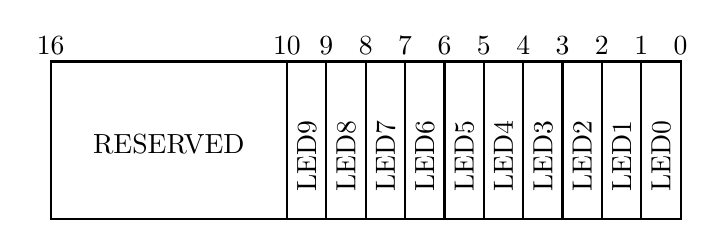
\begin{tikzpicture}[scale=1,line width=0.8pt] 
\coordinate (A16) at (0,0);
\coordinate (A10) at (3,0);
\coordinate (A9) at (3.5,0);
\coordinate (A8) at (4,0);
\coordinate (A7) at (4.5,0);
\coordinate (A6) at (5,0);
\coordinate (A5) at (5.5,0);
\coordinate (A4) at (6,0);
\coordinate (A3) at (6.5,0);
\coordinate (A2) at (7,0);
\coordinate (A1) at (7.5,0);
\coordinate (A0) at (8,0);
\coordinate (C) at (8,2);
\coordinate (D) at (0,2);
\draw(A16)--(A0)--(C)--(D)--cycle;
%the separator
\foreach \i/\texti  in {0,1,2,3,4,5,6,7,8,9,10} {
\draw (A\texti) to ($(A\texti)+(0,2)$);
}
%led
\foreach \i/\texti in {0,1,2,3,4,5,6,7,8,9} {
    \node[rotate=90] (LED\texti) at ($(A\texti) + (-0.25,0.8)$) {LED\texti};
}
%addr
\foreach \i/\texti in {0,1,2,3,4,5,6,7,8,9,10,16} {
    \node (ADDR\texti) at ($(A\texti) + (0,2.2)$) {\texti};
}
%reserved
\coordinate[label=below:RESERVED] (RESERVED) at ($(A16)!0.5!(A10) + (0,1.2)$);
\end{tikzpicture}
\section{显示驱动}
\subsection{VGA驱动}
\subsubsection{基本信息}
模块名:vga\_ctrl(内部模块)
\subsubsection{接口}
\begin{tabular}{|c|c|c|c|}
    \hline
    类型    &   位宽    &   名称    &   说明\\\hline
    input   &   1   &   pclk &   25MHz时钟\\\hline
    input   &   1   &   reset  &   置位\\\hline
    input   &   24   &   vga\_data  &   vga数据\\\hline
    output   &   10   &   h\_addr  &   水平方向扫描像素点坐标\\\hline
    output   &   10   &   v\_addr  &   垂直方向扫描像素点坐标\\\hline
    output   &   1   &   hsync  &   行同步信号\\\hline
    output   &   1   &   vsync  &   列同步信号\\\hline
    output   &   1   &   valid  &   消隐信号\\\hline
    output   &   8   &   vga\_r  &   R颜色信号\\\hline
    output   &   8   &   vga\_g  &   G颜色信号\\\hline
    output   &   8   &   vga\_b  &   B颜色信号\\\hline
\end{tabular}
\subsubsection{说明}
本模块提供底层VGA控制。
\subsection{显示驱动}
\subsubsection{基本信息}
模块名:display\_ctrl
\subsubsection{接口}
\begin{tabular}{|c|c|c|c|}
    \hline
    类型    &   位宽    &   名称    &   说明\\\hline
    input   &   1   &   clk &   50MHz时钟\\\hline
    input   &   1   &   reset\_n  &   复位\\\hline
    input   &   16   &   in\_data  &   输入数据\\\hline
    input   &   DP\_REG\_WIDTH   &   ctrl\_reg  &   控制寄存器\\\hline
    output   &   DP\_X\_ADDR\_WIDTH   &   x\_addr  &   水平坐标\\\hline
    output   &   DP\_Y\_ADDR\_WIDTH   &   y\_addr  &   垂直坐标\\\hline
    \multicolumn{4}{|c|}{硬件控制信号}\\\hline
    input   &   1   &   vga\_rst  &   VGA复位信号\\\hline
    output   &   1   &   vga\_vs  &   VGA列同步信号\\\hline
    output   &   1   &   vga\_hs  &   VGA行同步信号\\\hline
    output   &   1   &   vga\_syncn  &   VGA同步信号\\\hline
    output   &   1   &   vga\_blankn  &   VGA消隐信号\\\hline
    output   &   1   &   vga\_clk  &   VGA时钟信号\\\hline
    output   &   8   &   vga\_r  &   VGA R颜色信号\\\hline
    output   &   8   &   vga\_g  &   VGA G颜色信号\\\hline
    output   &   8   &   vga\_b  &   VGA B颜色信号\\\hline
\end{tabular}
\subsubsection{说明}
本模块提供显示控制驱动。输入数据in\_data中,低8位为ASCII码,高8位为颜色数据,其中,高4位为前景色,低4位为背景色。
\subsubsection{控制寄存器}
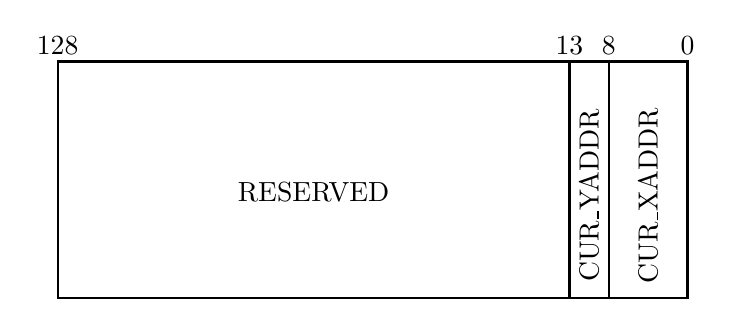
\begin{tikzpicture}[scale=1,line width=0.8pt] 
\coordinate (A8) at (0,0);
\coordinate (YADDRA) at (6.5,0);
\coordinate (XADDRA) at (7,0);
\coordinate (A0) at (8,0);
\coordinate (C) at (8,3);
\coordinate (D) at (0,3);
\draw(A8)--(A0)--(C)--(D)--cycle;
%the separator
\draw (XADDRA) to ($(XADDRA)+(0,3)$);
\draw (YADDRA) to ($(YADDRA)+(0,3)$);
%label
\node[rotate=90] (CURXADDR) at ($(A0) + (-0.5,1.3)$) {CUR\_XADDR};
\node[rotate=90] (CURYADDR) at ($(XADDRA) + (-0.25,1.3)$) {CUR\_YADDR};
%addr
\node (A0ADDR) at ($(A0) + (0,3.2)$) {0};
\node (XADDR) at ($(XADDRA) + (0,3.2)$) {8};
\node (YADDR) at ($(YADDRA) + (0,3.2)$) {13};
\node (A8ADDR) at ($(A8) + (0,3.2)$) {128};
%reserved
\coordinate[label=below:RESERVED] (RESERVED) at ($(A8)!0.5!(YADDRA) + (0,1.6)$);
\end{tikzpicture}\\
其中,CUR\_XADDR和CUR\_YADDR代表当前光标位置。
\subsubsection{颜色表}
\begin{tabular}{|c|c|c|}
    \hline
    名称 & 值 & 说明\\\hline
    \multicolumn{3}{|c|}{颜色代码}\\\hline
    VGA\_BLACK & 0x0 & 黑\\\hline
    VGA\_BLUE & 0x1 & 蓝\\\hline
    VGA\_GREEN & 0x2 & 绿\\\hline
    VGA\_CYAN & 0x3 & 青\\\hline
    VGA\_RED & 0x4 & 红\\\hline
    VGA\_MAGENTA & 0x5 & 洋红\\\hline
    VGA\_BROWN & 0x6 & 棕\\\hline
    VGA\_WHITE & 0x7 & 白\\\hline
    VGA\_YELLOW & 0xe & 黄\\\hline
    \multicolumn{3}{|c|}{对应RGB}\\\hline
    VGA\_RGB\_BLACK & 000000 & 黑\\\hline
    VGA\_RGB\_BLUE & 0000ff & 蓝\\\hline
    VGA\_RGB\_GREEN & 008000 & 绿\\\hline
    VGA\_RGB\_CYAN & 00ffff & 青\\\hline
    VGA\_RGB\_RED & ff0000 & 红\\\hline
    VGA\_RGB\_MAGENTA & ff00ff & 洋红\\\hline
    VGA\_RGB\_BROWN & a52a2a & 棕\\\hline
    VGA\_RGB\_WHITE & ffffff & 白\\\hline
    VGA\_RGB\_YELLOW & ffff00 & 黄\\\hline
\end{tabular}\\

\subsubsection{字符扩展}
\begin{tabular}{|c|c|}
    \hline
    编码 & 说明\\\hline
    0x1	&实心方框\\\hline
    0x2	&上半实心方框\\\hline
    0x3	&下半实心方框\\\hline
    0x4	&实心圆\\\hline
    0x5	&上三角形\\\hline
    0x6	&右三角形\\\hline
    0x7	&右上三角形\\\hline
    0xe	&右下三角形\\\hline
    0xf	&左三角形\\\hline
    0x10&	左上三角形\\\hline
    0x11&	左下三角形\\\hline
    0x12&	下三角形\\\hline
\end{tabular}\\
\part{软件}
%
% Copyright 2018 EmmmHackers
% 
% 
% Licensed under the Apache License, Version 2.0 (the "License");
% you may not use this file except in compliance with the License.
% You may obtain a copy of the License at
% 
% 
%       http://www.apache.org/licenses/LICENSE-2.0
% 
% 
% Unless required by applicable law or agreed to in writing, software
% distributed under the License is distributed on an "AS IS" BASIS,
% WITHOUT WARRANTIES OR CONDITIONS OF ANY KIND, either express or implied.
% See the License for the specific language governing permissions and
% limitations under the License.
% --------------------------
% File: kernel_introduction.tex
% Project: EmmmCS
% File Created: 2018-12-07 19:23:25
% Author: Chen Haodong (easyai@outlook.com)
% --------------------------
% Last Modified: 2018-12-08 16:41:41
% Modified By: Chen Haodong (easyai@outlook.com)
%
\chapter{Kernel 综述}
\section{架构}
本Kernel不提供进程、线程模型,文件系统,网络。\\
本Kernel由以下部分组成:
\begin{itemize}
    \item KLIB - Kernel编程的基础库
    \item driver - 提供对VGA、PS/2 KB、LED等设备控制
    \item mm - 内存管理器,提供动态内存管理
    \item sh - 提供交互式命令行
    \item app - 内置应用
\end{itemize}
\section{常量、类型}
\begin{tabular}{|c|c|c|}
    \hline
    名称 & 值 & 说明\\\hline
    NULL & 0 & NULL值\\\hline
    FALSE & 0 & 布尔False\\\hline
    TRUE & 1 & 布尔True\\\hline
\end{tabular}\\
\begin{tabular}{|c|c|c|}
    \hline
    名称 & 对应类型 & 说明\\\hline
    BOOL & unsigned char & 布尔类型\\\hline
    u8 & unsigned char & 8位无符号数\\\hline
    u16 & unsigned short & 16位无符号数\\\hline
    u32 & unsigned int & 32位无符号数\\\hline
    s8 & char & 8位有符号数\\\hline
    s16 & short & 16位有符号数\\\hline
    s32 & int & 32位有符号数\\\hline
\end{tabular}
%
% Copyright 2018 EmmmHackers
%
%
% Licensed under the Apache License, Version 2.0 (the "License");
% you may not use this file except in compliance with the License.
% You may obtain a copy of the License at
%
%
%       http://www.apache.org/licenses/LICENSE-2.0
%
%
% Unless required by applicable law or agreed to in writing, software
% distributed under the License is distributed on an "AS IS" BASIS,
% WITHOUT WARRANTIES OR CONDITIONS OF ANY KIND, either express or implied.
% See the License for the specific language governing permissions and
% limitations under the License.
% --------------------------
% File: kernel_intr.tex
% Project: EmmmCS
% File Created: 2018-12-08 16:58:40
% Author: Chen Haodong (easyai@outlook.com)
%         Xie Nairong (jujianai@hotmail.com)
% --------------------------
% Last Modified: 2018-12-08 17:15:10
% Modified By: Chen Haodong (easyai@outlook.com)
%

\chapter{Kernel 中断处理}
中断规定、中断表见CPU中断部分。\textbf{注意Kernel统一将中断处理函数设置为intr,通过在intr内部读取中断号进行中断分发,不再由CPU进行中断分发}
\section{intr\_init}
\texttt{void intr\_init(void)}

简介:对中断模块进行初始化。

\subsection{函数功能}

开机时被调用,初始化中断模块。

\section{intr\_open}
\texttt{void intr\_open(void)}

简介:打开中断。

\section{intr\_close}
\texttt{void intr\_close(void)}

简介:关闭中断。

\section{intr}
\texttt{void intr(void)}

简介:中断处理主函数,用于分发中断。

\section{intr\_handler\_register}
\texttt{void intr\_handler\_register(u8 intrno, void *handler)}

简介:对相应中断处理函数进行注册。
%
% Copyright 2018 EmmmHackers
%
%
% Licensed under the Apache License, Version 2.0 (the "License");
% you may not use this file except in compliance with the License.
% You may obtain a copy of the License at
%
%
%       http://www.apache.org/licenses/LICENSE-2.0
%
%
% Unless required by applicable law or agreed to in writing, software
% distributed under the License is distributed on an "AS IS" BASIS,
% WITHOUT WARRANTIES OR CONDITIONS OF ANY KIND, either express or implied.
% See the License for the specific language governing permissions and
% limitations under the License.
% --------------------------
% File: kernel_driver.tex
% Project: EmmmCS
% File Created: 2018-12-08 16:21:25
% Author: Chen Haodong (easyai@outlook.com)
% --------------------------
% Last Modified: 2018-12-08 16:45:42
% Modified By: Chen Haodong (easyai@outlook.com)
%

\chapter{Kernel 驱动}
\section{LED}
LED使用2个字节的控制寄存器,内存映射在0x80000起始。
\subsection{接口}

\subsubsection{led\_init}
\noindent函数原型:void led\_init(void);\\
说明:led驱动初始化

\subsubsection{led\_on}
\noindent函数原型:void led\_on(u8 id);\\
参数:\\
\begin{tabular}{|c|c|c|}
    \hline
    类型 & 名称 & 说明\\\hline
    u8 & id & 取值0-9,对应led的id\\\hline
\end{tabular}\\
说明:开对应led,若id非法,无操作。

\subsubsection{led\_off}
\noindent函数原型:void led\_off(u8 id);\\
参数:\\
\begin{tabular}{|c|c|c|}
    \hline
    类型 & 名称 & 说明\\\hline
    u8 & id & 取值0-9,对应led的id\\\hline
\end{tabular}\\
说明:关对应led,若id非法,无操作。

\subsubsection{led\_toggle}
\noindent函数原型:void led\_toggle(u8 id);\\
参数:\\
\begin{tabular}{|c|c|c|}
    \hline
    类型 & 名称 & 说明\\\hline
    u8 & id & 取值0-9,对应led的id\\\hline
\end{tabular}\\
说明:反转对应led状态,若id非法,无操作。

\section{VGA}
屏幕坐标,以左上角为原点,横向为x轴,纵向为y轴。
\subsection{常量、宏、类型}
\noindent\begin{tabular}{|c|c|c|}
    \hline
    名称 & 值 & 说明\\\hline
    VGA\_CHAR\_X\_SIZE & 80 & 列数\\\hline
    VGA\_CHAR\_Y\_SIZE & 30 & 行数\\\hline
    VGA\_CHAR\_BUF\_SIZE & 2400 & 总字符数\\\hline
\end{tabular}\\
\begin{tabular}{|c|c|c|}
    \hline
    名称 & 值 & 说明\\\hline
    \multicolumn{3}{|c|}{背景色}\\\hline
    VGA\_B\_BLACK & 0x00 & 黑\\\hline
    VGA\_B\_BLUE & 0x10 & 蓝\\\hline
    VGA\_B\_GREEN & 0x20 & 绿\\\hline
    VGA\_B\_CYAN & 0x30 & 青\\\hline
    VGA\_B\_RED & 0x40 & 红\\\hline
    VGA\_B\_MAGENTA & 0x50 & 洋红\\\hline
    VGA\_B\_BROWN & 0x60 & 棕\\\hline
    VGA\_B\_WHITE & 0x70 & 白\\\hline
    \multicolumn{3}{|c|}{前景色}\\\hline
    VGA\_F\_BLACK & 0x00 & 黑\\\hline
    VGA\_F\_BLUE & 0x01 & 蓝\\\hline
    VGA\_F\_GREEN & 0x02 & 绿\\\hline
    VGA\_F\_CYAN & 0x03 & 青\\\hline
    VGA\_F\_RED & 0x04 & 红\\\hline
    VGA\_F\_MAGENTA & 0x05 & 洋红\\\hline
    VGA\_F\_BROWN & 0x06 & 棕\\\hline
    VGA\_F\_WHITE & 0x07 & 白\\\hline
    \multicolumn{3}{|c|}{数字格式}\\\hline
    VGA\_N\_S\_DEC & 0x0 & 有符号十进制\\\hline
    VGA\_N\_U\_DEC & 0x1 & 无符号十进制\\\hline
    VGA\_N\_HEX & 0x2 & 十六进制\\\hline
\end{tabular}\\
\subsection{接口}

\subsubsection{vga\_init}
\noindent函数原型:void vga\_init(void);\\
说明:vga驱动初始化

\subsubsection{vga\_writec}
\noindent函数原型:void vga\_writec(u8 color, char c, u8 x, u8 y);\\
参数:\\
\begin{tabular}{|c|c|c|}
    \hline
    类型 & 名称 & 说明\\\hline
    u8 & color & 颜色\\\hline
    char & c & 输出字符\\\hline
    u8 & x & x坐标\\\hline
    u8 & y & y坐标\\\hline
\end{tabular}\\
说明:在对应坐标处写入字符,若坐标非法则无操作。注意该函数不改变光标位置。

\subsubsection{vga\_putc}
\noindent函数原型:void vga\_putc(u8 color, char c);\\
参数:\\
\begin{tabular}{|c|c|c|}
    \hline
    类型 & 名称 & 说明\\\hline
    u8 & color & 颜色\\\hline
    char & c & 输出字符\\\hline
\end{tabular}\\
说明:在光标处写入字符,该函数会自动滚屏。

\subsubsection{vga\_puts}
\noindent函数原型:void vga\_puts(u8 color, const char *str);\\
参数:\\
\begin{tabular}{|c|c|c|}
    \hline
    类型 & 名称 & 说明\\\hline
    u8 & color & 颜色\\\hline
    const char* & str & 输出字符串\\\hline
\end{tabular}\\
说明:在光标处写入字符串,该函数会自动滚屏。

\subsubsection{vga\_putn}
\noindent函数原型:void vga\_putn(u8 color, u32 n, u8 mode);\\
参数:\\
\begin{tabular}{|c|c|c|}
    \hline
    类型 & 名称 & 说明\\\hline
    u8 & color & 颜色\\\hline
    u32 & n & 输出数字\\\hline
    u8 & mode & 数字格式\\\hline
\end{tabular}\\
说明:在光标处写入数字,该函数会自动滚屏。

\subsubsection{vga\_clean}
\noindent函数原型:void vga\_clean(void);\\
说明:清屏

\section{KBD}
KBD 维护一个环形字符缓冲区。

\subsection{接口}

\subsubsection{kbd\_update}
\noindent函数原型:void kbd\_update(u8* args);\\

使用一个两字节的内存空间维护键盘状态,cpu 在中断前应写好对应地址内容

\begin{tabular}{|c|c|}
    \hline
    参数 & 含义 \\\hline
    \texttt{args[0]} & 是否有效 \\\hline
    \texttt{args[1]} & 键盘扫描码 \\\hline
\end{tabular}

说明:中断处理函数,在键盘按下时被调用;作用是把键盘操作写入缓冲区。

\subsubsection{kbd\_getc}
\noindent函数原型:u8 kbd\_getc();\\
说明:从缓冲区读取一位字符 ascii 码并返回。

%
% Copyright 2018 EmmmHackers
%
%
% Licensed under the Apache License, Version 2.0 (the "License");
% you may not use this file except in compliance with the License.
% You may obtain a copy of the License at
%
%
%       http://www.apache.org/licenses/LICENSE-2.0
%
%
% Unless required by applicable law or agreed to in writing, software
% distributed under the License is distributed on an "AS IS" BASIS,
% WITHOUT WARRANTIES OR CONDITIONS OF ANY KIND, either express or implied.
% See the License for the specific language governing permissions and
% limitations under the License.
% --------------------------
% File: kernel_lib.tex
% Project: EmmmCS
% File Created: 2018-12-08 16:58:40
% Author: Chen Haodong (easyai@outlook.com)
% --------------------------
% Last Modified: 2018-12-08 17:15:10
% Modified By: Chen Haodong (easyai@outlook.com)
%

\chapter{Kernel Lib}
若函数与C标准库中函数同名,则其行为也一致。该部分函数文档见C11标准文档。

\section{DList}
提供了侵入式双向链表。链表头结点不存放数据。

\subsection{接口}

\subsubsection{DLIST\_INIT}
\noindent{函数原型:DLIST\_INIT(list, m\_next, m\_prev)}\\
参数:\\
\begin{tabular}{|c|c|c|}
    \hline
    类型 & 名称 & 说明\\\hline
    ptr & list & 链表头结点\\\hline
    member name & m\_next & 后驱变量名\\\hline
    member name & m\_prev & 前驱变量名\\\hline
\end{tabular}\\
说明:初始化链表

\subsubsection{DLIST\_EMPTY}
\noindent{函数原型:DLIST\_EMPTY(list, m\_next, m\_prev)}\\
参数:\\
\begin{tabular}{|c|c|c|}
    \hline
    类型 & 名称 & 说明\\\hline
    ptr & list & 链表头结点\\\hline
    member name & m\_next & 后驱变量名\\\hline
    member name & m\_prev & 前驱变量名\\\hline
\end{tabular}\\
说明:判断链表是否为空

\subsubsection{DLIST\_INSERT}
\noindent{函数原型:DLIST\_INSERT(pos, m\_next, m\_prev, node)}\\
参数:\\
\begin{tabular}{|c|c|c|}
    \hline
    类型 & 名称 & 说明\\\hline
    ptr & pos & 被插入结点的前驱\\\hline
    member name & m\_next & 后驱变量名\\\hline
    member name & m\_prev & 前驱变量名\\\hline
    ptr & node & 被插入结点\\\hline
\end{tabular}\\
说明:插入结点


\subsubsection{DLIST\_DELETE}
\noindent{函数原型:DLIST\_DELETE(list, pos, m\_next, m\_prev)}\\
参数:\\
\begin{tabular}{|c|c|c|}
    \hline
    类型 & 名称 & 说明\\\hline
    ptr & list & 链表\\\hline
    ptr & pos & 被删除结点\\\hline
    member name & m\_next & 后驱变量名\\\hline
    member name & m\_prev & 前驱变量名\\\hline
\end{tabular}\\
说明:删除结点

\subsubsection{DLIST\_ADD\_TAIL}
\noindent{函数原型:DLIST\_ADD\_TAIL(list, m\_next, m\_prev, node)}\\
参数:\\
\begin{tabular}{|c|c|c|}
    \hline
    类型 & 名称 & 说明\\\hline
    ptr & list & 链表\\\hline
    member name & m\_next & 后驱变量名\\\hline
    member name & m\_prev & 前驱变量名\\\hline
    ptr & node & 被添加结点\\\hline
\end{tabular}\\
说明:添加结点至链表尾

\subsubsection{DLIST\_ADD\_HEAD}
\noindent{函数原型:DLIST\_ADD\_HEAD(list, m\_next, m\_prev, node)}\\
参数:\\
\begin{tabular}{|c|c|c|}
    \hline
    类型 & 名称 & 说明\\\hline
    ptr & list & 链表\\\hline
    member name & m\_next & 后驱变量名\\\hline
    member name & m\_prev & 前驱变量名\\\hline
    ptr & node & 被添加结点\\\hline
\end{tabular}\\
说明:添加结点至链表头

\subsubsection{DLIST\_FOREACH}
\noindent{函数原型:DLIST\_FOREACH(list, m\_next, ptr)}\\
参数:\\
\begin{tabular}{|c|c|c|}
    \hline
    类型 & 名称 & 说明\\\hline
    ptr & list & 链表\\\hline
    member name & m\_next & 后驱变量名\\\hline
    ptr & ptr & 当前操作结点\\\hline
\end{tabular}\\
说明:链表遍历

\subsubsection{DLIST\_FIND\_NODE}
\noindent{函数原型:DLIST\_FIND\_NODE(list, m\_next, p\_node, key, cmpfunc)}\\
参数:\\
\begin{tabular}{|c|c|c|}
    \hline
    类型 & 名称 & 说明\\\hline
    ptr & list & 链表\\\hline
    member name & m\_next & 后驱变量名\\\hline
    ptr & p\_node & 返回值\\\hline
    value & key & 关键字\\\hline
    function & cmpfunc & 比较函数\\\hline
\end{tabular}\\
比较函数要求:二元函数,左操作数接受key值,右操作数接受一个指向链表结点的指针,若匹配返回非零值。\\
说明:链表结点查找,若查找不到返回NULL。

\section{stdio}

\subsection{接口}

\subsubsection{getchar}
\noindent{函数原型:\texttt{char getchar(void);}} \\
从键盘读取一个字符,返回其 ascii 码。

\subsubsection{gets}
\noindent{函数原型:\texttt{char* gets(char* str);}} \\
从键盘读取一个字符串,写入 \texttt{str} 中,以 \begin{verbatim}'\0'\end{verbatim} 结尾。\\
返回值为 \texttt{str}。

\subsubsection{putchar}
\noindent{函数原型:\texttt{int putchar(char cha);}} \\
将 \texttt{cha} 输出到 vga 缓冲区。

\subsubsection{puts}
\noindent{函数原型:\texttt{int puts(const char* str);}} \\
将字符串 \texttt{str} 输出到 vga 缓冲区。

\subsubsection{putn}
\noindent{函数原型:\texttt{void putn(u32 n, u8 mode);}} \\

参数说明:

\begin{tabular}{|c|c|c|}
    \hline
    类型 & 名称 & 说明\\\hline
    u32 & n & 输出数字\\\hline
    u8 & mode & 数字格式\\\hline
\end{tabular}

\subsubsection{putchar\_color}
\noindent{函数原型:\texttt{int putchar\_color(u8 color, char cha);} }\\
将 \texttt{cha} 输出到 vga 缓冲区,带有颜色 \texttt{color}。

\subsubsection{puts\_color}
\noindent{函数原型:\texttt{int puts\_color(u8 color, const char * str);}} \\
将字符串 \texttt{str} 输出到 vga 缓冲区,带有颜色 \texttt{color}。


\subsubsection{putn\_color}
\noindent{函数原型:\texttt{void putn\_color(u8 color, u32 n, u8 mode);} }\\
\begin{tabular}{|c|c|c|}
    \hline
    类型 & 名称 & 说明\\\hline
    u8 & color & 颜色\\\hline
    u32 & n & 输出数字\\\hline
    u8 & mode & 数字格式\\\hline
\end{tabular}\\
%
% Copyright 2018 EmmmHackers
% 
% 
% Licensed under the Apache License, Version 2.0 (the "License");
% you may not use this file except in compliance with the License.
% You may obtain a copy of the License at
% 
% 
%       http://www.apache.org/licenses/LICENSE-2.0
% 
% 
% Unless required by applicable law or agreed to in writing, software
% distributed under the License is distributed on an "AS IS" BASIS,
% WITHOUT WARRANTIES OR CONDITIONS OF ANY KIND, either express or implied.
% See the License for the specific language governing permissions and
% limitations under the License.
% --------------------------
% File: kernel_mm.tex
% Project: EmmmCS
% File Created: 2018-12-08 16:46:37
% Author: Chen Haodong (easyai@outlook.com)
% --------------------------
% Last Modified: 2018-12-08 16:57:15
% Modified By: Chen Haodong (easyai@outlook.com)
%

\chapter{Kernel 内存管理}
Kernel 提供128KB的堆内存管理,采用Buddy Memory Management。

\section{常量、宏、类型}
\noindent\begin{tabular}{|c|c|c|}
    \hline
    名称 & 值 & 说明\\\hline
    HEAP\_SIZE & 131072 & 128KB\\\hline
    TREE\_DEPTH & 14 & 分配粒度\\\hline
\end{tabular}\\

\subsubsection{buddy\_mm\_info\_t}
\noindent成员:\\
\begin{tabular}{|c|c|c|}
    \hline
    类型 & 名称 & 说明\\\hline
    buddy\_mm\_info\_t* & m\_next & 链表,后驱\\\hline
    buddy\_mm\_info\_t* & m\_prev & 链表,前驱\\\hline
\end{tabular}\\
说明:空闲块链表项。

\subsubsection{buddy\_mm\_header\_t}
\noindent类型:u32\\
说明:指针Header,存储level

\subsubsection{buddy\_mm\_t}
\noindent成员:\\
\begin{tabular}{|c|c|c|}
    \hline
    类型 & 名称 & 说明\\\hline
    u32 & used\_size & 已使用大小\\\hline
    buddy\_mm\_info\_t*[TREE\_DEPTH] & tree & 空闲块集合\\\hline
\end{tabular}\\
说明:Buddy内存分配系统。

\section{接口}

\subsubsection{mm\_init}
\noindent函数原型:void mm\_init(void);\\
说明:内存管理初始化。

\subsubsection{mm\_alloc}
\noindent函数原型:void* mm\_alloc(u32 sz);\\
参数:\\
\begin{tabular}{|c|c|c|}
    \hline
    类型 & 名称 & 说明\\\hline
    u32 & sz & 需分配大小\\\hline
\end{tabular}\\
返回值:内存块起始地址,若分配失败返回NULL\\
说明:内存块分配。

\subsubsection{mm\_dealloc}
\noindent函数原型:void mm\_dealloc(void *p);\\
参数:\\
\begin{tabular}{|c|c|c|}
    \hline
    类型 & 名称 & 说明\\\hline
    void* & p & 需回收内存块指针\\\hline
\end{tabular}\\
说明:回收相应内存块。
\end{sloppypar}
\end{document}